\chapter[Lecture 20]{}\label{lec20}

$$
\fbox{$\theta=\dfrac{\hbar w_{D}}{k_{B}}=\dfrac{\hbar \nu_{D}}{k_{B}}\left(\dfrac{6\pi^{2}N}{V}\right)^{\frac{1}{3}}$}
$$
\begin{align*}
\Lt\limits_{x\to 0}\dfrac{x^{4}e^{x}}{(e^{x}-1)^{2}} &= \Lt\limits_{x\to 0}\dfrac{4x^{3}}{2e^{x}(e^{x}-1)}=\Lt\limits_{x\to 0}\dfrac{x^{2}}{e^{x}}\\[3pt]
\Lt\limits_{x\to 0}\dfrac{x^{2}e^{x}}{(e^{x}-1)^{2}} &= \Lt\limits_{x\to 0}\dfrac{2x}{2e^{x}(e^{x}-1)}=\Lt\limits_{x\to 0}\dfrac{x}{e^{x}-1}=1\\[3pt]
\therefore \ U &= 9Nk_{B}T\left(\dfrac{T}{\theta}\right)^{3}\int\limits^{x_{D}}_{0}dx\cdot \dfrac{x^{3}}{e^{x}-1}\quad x_{D}=\dfrac{\theta}{T}\\[3pt]
C_{V} &= \dfrac{3V\hbar}{2\pi^{2}\nu^{3}}\cdot \dfrac{\hbar}{k_{B}T^{2}}\int\limits^{w_{D}}_{0}dw\dfrac{w^{4}e^{\beta\hbar w}}{(e^{\beta\hbar w}-1)^{2}}=9Nk_{B}\left(\dfrac{I}{\theta}\right)^{3}\int\limits^{x_{D}}_{0}dx\dfrac{x^{4}e^{x}}{(e^{x}-1)^{2}}
\end{align*}
for $T\gg \theta$\quad $C_{V}\simeq 3Nk_{B}$
$$
9Nk_{B}\left(\dfrac{T}{\theta}\right)^{3}\int\limits^{x_{D}}_{0}dx\cdot x^{2}=9Nk_{B}\left(\dfrac{T}{\theta}\right)^{3}\cdot \left.\dfrac{x^{3}}{3}\right]^{x_{D}}_{0}=3Nk_{B}.
$$
$C_{V}$ approaches classical value.

at $T$ very small $x_{D}\to \infty$.
\begin{align*}
\therefore\quad \int\limits^{\infty}_{0}dx\cdot \dfrac{x^{3}}{e^{x}-1} &=\int\limits^{\infty}_{0}dx\cdot x^{3}\sum\limits^{\infty}_{s=1}e^{-Sx}=6\sum\limits^{\infty}_{S=1}\dfrac{1}{S^{4}}=\dfrac{\pi^{4}}{15}\\[3pt]
\Rightarrow \sum\limits^{\infty}_{1}\dfrac{1}{S^{4}} &= \dfrac{\pi^{4}}{90}\text{ found from table.}
\end{align*}
$\therefore \ U\simeq \dfrac{3\pi^{4}Nk_{B}T^{4}}{5\theta^{3}}$
$$
\therefore \ \fbox{$C_{V}=\dfrac{12\pi^{4}}{5}\cdot Nk_{B}\left(\dfrac{T}{\theta}\right)^{3}$} \simeq 234Nk_{B}\left(\dfrac{T}{\theta}\right)^{3}\Leftarrow \text{Debye's $T^{3}$-law.}
$$
\begin{itemize}
\itemsep=0pt
\item[$\to$] $T^{3}$ approximation is quite good at very low temperature as only the long wavelength acoustic moes are excited.

\item[$\to$] Short wavelength modes have too high energy to be populated at low temperatures, Hence, the continuum approximation holds good at low $T$.

\item[$\to$] For real systems $T^{3}$ works for $T\lesssim \dfrac{\theta}{50}$
\end{itemize}

\noindent
{\bf Einstein's model (1907):} Introduced the concept of energy quanta for lattice vibrations as phonons in analogy of photons.

\section*{Postulates}
\begin{itemize}
\itemsep=0pt
\item[(i)] All atoms in a solid vibrates at a fixed frequency, $\nu$. Energy is not continuous, it is $E=nh\nu$; $\epsilon=h\nu$ is the energy of quasiparticle, phonon.

\item[(ii)] Used statistical physics to calculate energy distribution, specially Boltzmann principle $S=k_{B}ln\Omega$
\begin{quote}
$S=$ entropy, $k_{B}=$ Boltzmann constant

$\Omega=$ No. of available microscopic states
\end{quote}
At temp. $T$, $3N$ fold degenerate level, $\epsilon=h\nu$, Average no. of phonons $\overline{n}$, can be calculated by minimizing the grans potential $J=U-TS-\mu N$ or {\em Landau free energy}, $\mu=$ Chemical potential.

$=F \text{(Helmboltz free energy)} -G \text{(Gibb's free energy)}$ 
$$
G=U+pV-TS=\sum\mu_{1}N_{i}\text{~ for a homogeneous system}
$$
\end{itemize}

$\mu=0$ due to non-conservation of phonon numbers in Bose gas.
\begin{align*}
\therefore\quad 0 &=\dfrac{dJ}{dn}=\dfrac{d}{dn}\left\{n\epsilon-k_{B^{T}}ln \dfrac{(n+3N)!}{n!(3N)!}\right\}/n=\overline{n}\\
&= \epsilon  k_{B^{T}}ln \dfrac{\overline{n}+3N}{\overline{n}}
\end{align*}
$$
\therefore\quad \fbox{$\hbar = 3N \dfrac{1}{e^{\epsilon/k_{B^{T}}}-1}$}=3N \ f_{B.E.}(\epsilon) \text{ (Base-Einstein distance function)}
$$

$\therefore$ The total energy 
$$
\fbox{$U=\dfrac{3N\hbar w}{e^{\beta\hbar w}-1}$}
$$
$$
\therefore \ C_{V}=\dfrac{\partial U}{\partial T}=3Nk_{B}\left(\dfrac{\theta_{E}}{T}\right)^{2}\dfrac{e^{\theta_{E}/T}}{(e^{\theta_{E}/T}-1)^{2}}
$$
where, \fbox{$\theta_{E}=\dfrac{\hbar w}{k_{B}}$} is called {\em Einstein temperature}, a characteristic constant of a certain solid.
\begin{align*}
C_{V} &\simeq 3Nk_{B}\left[1-\frac{1}{12}\left(\dfrac{\theta_{E}}{T}\right)^{2}\right]\quad\text{for}\quad T\gg \theta_{E}\\
&\simeq 3Nk_{B}\left(\dfrac{\theta_{E}}{T}\right)^{2}e^{-\frac{\theta_{E}}{T}}\quad\text{for}\quad T\ll \theta_{E}
\end{align*}

High temperature value tend to Dulong-Petit law. Low temperature limit show exponential change. At this level Debye model of $T^{3}$-dependence is more close to experiments.

\section*{Einstein temperature\quad \fbox{\protect\boldmath$\theta_{E}=\dfrac{h_{\nu}}{k_{B}}$}}
\begin{figure}[H]
\centering
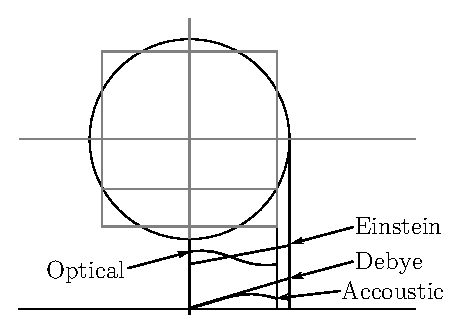
\includegraphics{images/lecture20/fig2.eps}
\end{figure}
$\theta_{E}$ is a characteristic constant in a solid, and related to the energy of phonons.

\section*{Debye Temperature}
$$
\theta_{D}=\dfrac{\hbar \nu}{k_{B}}\left(\dfrac{6\pi^{2}N}{V}\right)^{\frac{1}{3}}\quad \nu\to \text{velocity of sound.}
$$
Debye temperature plays the same role in lattice vibrations as the Fermi temperature $(T_{F})$ does in the theory of electrons in metals.

Both separates the low temperature region, where quantum theory is necessary to the high temperature region, where classical theory is adequate.

$T_{P}\sim 10^{3}K$ But $\theta_{D}\sim 10^{2}K$.

\section*{Analogy with black body radiation}

Correspondence between electro-magnetic theory of radiation at thermal equilibrium and theory of lattice vibrations.

Problem with classical description $\to$ All normal modes should contribute $k_{B}T$ to the energy.

Dulong-Petit's law is slightly better, as finit size of the solid allows some discrete values of $k\to$ finite number.
\begin{center}
\renewcommand{\arraystretch}{1.5}
\begin{tabular}{rlcc}
\hline
 & \multicolumn{1}{c}{\bf Differences} & {\bf Phonons} & {\bf Photons}\\
\hline
(i) & No. of Normal modes & $3n_{a}$ for each $\overrightarrow{k}$ & Two modes for each $k$\\
    &                     &                                       & (longitudinal is absent)\\[5pt]
(ii) & Restriction of $k$ & $-\dfrac{\pi}{a}\leq k\leq \dfrac{\pi}{a}$ & $\overrightarrow{k}$ arbitrary\\[10pt]
(iii) & Thermal energy density & $\sum\limits_{S}\int\limits^{k_{D}}\dfrac{d\overrightarrow{k}}{(2\pi)^{3}}\dfrac{hw_{S}(k)}{e^{\partial \hbar w_{S}(k)}-1}$ & $2\int\limits^{\infty}\dfrac{d\overrightarrow{k}}{(2\pi)^{3}}\dfrac{\hbar ck}{e^{\beta \hbar ck}-1}$\\
\hline
\end{tabular}
\end{center}
No restriction on $k$.

\section*{Density of states}

No. of states per unit frequency range, given the phonon dispersion $w(k)$
$$
D(w)dw=\int\limits_{\text{shell}}\left(\dfrac{L}{2\pi}\right)^{3}\cdot d^{3}k=\left(\dfrac{L}{2\pi}\right)^{3}\int\limits_{\text{shell}}d^{3}k
$$

The problem is to evaluate the volume of the shell.

Assume $dS_{w}$ denote the area element on the surface of $k$-space
\begin{figure}[H]
\centering
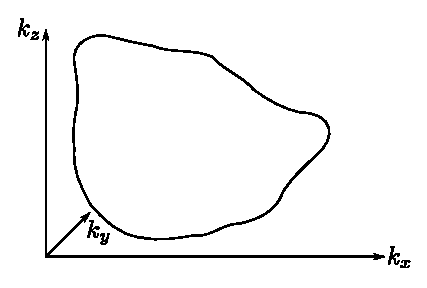
\includegraphics[scale=.9]{images/lecture20/fig3.eps}
\end{figure}
$$
\therefore\quad \int d^{3}k=\int dS_{w}dk_{\perp}
$$
$dk_{\perp}$ is the perpendicular distance between $w$ and $w+dw$ surfaces.
\begin{gather*}
\therefore\quad \left|\nabla_{k}w\right| dk_{\perp}=dw\\[2pt]
\therefore\quad dS_{w}dk_{\perp}=dS_{w}\dfrac{dw}{|\nabla_{k}w|}=dS_{w}\dfrac{dw}{v_{g}}\\[2pt]
v_{g}=|\nabla_{k}w|=\text{ group velocity of a phonon}\\[2pt]
\therefore \ D(w)dw=\left(\dfrac{L}{2\pi}\right)^{3}\int \dfrac{dS_{w}dw}{v_{g}}=\dfrac{V}{(2\pi)^{3}}\int \dfrac{dS_{w}}{v_{g}}dw\\[2pt]
\therefore \quad \fbox{$D(w)=\dfrac{V}{(2\pi)^{3}}\int \dfrac{dS_{w}}{v_{g}}$}
\end{gather*}
\begin{itemize}
\item This result refers to a single branch of the dispersion relation.

\item When $v_{g}$ is zero, $D(w)$ has a singularity called {\em Van Hore singularity}
\begin{figure}[H]
\centering
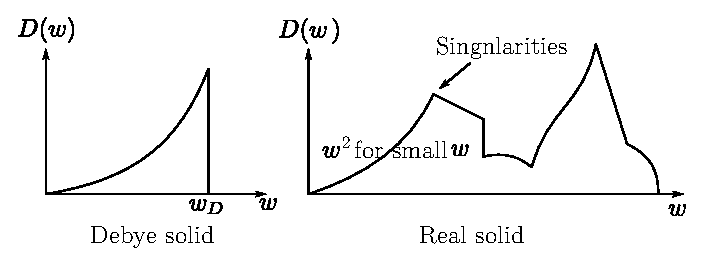
\includegraphics{images/lecture20/fig4.eps}
\end{figure}
\end{itemize}

\section*{Anharmonic Interactions}

\subsection*{Harmonic approximation}
\begin{itemize}
\itemsep=0pt
\item[(i)] Two lattice wave do not interact with each other; a single wave does not decay or change form with time.

\item[(ii)] There is no thermal expansion.

\item[(iii)] Adiabatic and Isothermal elastic constants are equal.

\item[(iv)] The elastic constants are independent of pressure and temperature.

\item[(v)] Heat capacity becomes constant at $T>\theta_{D}$.
\end{itemize}
Real solids are very different - The deviations are attributed to the anharmonicity of the system.

Experiment shows that interaction of two phonons can produce a third one, $w_{3}=w_{1}+w_{2}$. This requires higher order terms in the interaction potential.

\subsection*{Thermal expansion}

The anharmonicity in the interaction potential leads to displacement from equillibrium position, which is expansion/compression.
\begin{figure}[H]
\centering
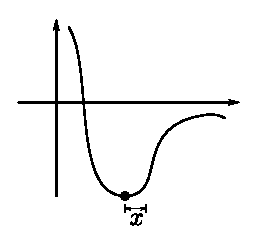
\includegraphics{images/lecture20/fig5.eps}
\end{figure}

For the displacement `$n$'
$$
v(x)=cx^{2}-gx^{3}-fx^{y}
$$
$c$, $g$, $f$ are positive.
\begin{itemize}
\itemsep=0pt
\item[$\to$] $x^{3}$-term represents asymmetry of the mutual repulsion of atoms.

\item[$\to$] $x^{4}$-term represents softening of the vibration at large amplitudes.
\end{itemize}
Using Boltzmann distribution
$$
\langle x \rangle = \dfrac{\int\limits^{\infty}_{-\infty}dx\cdot x\cdot e^{-\beta U(x)}}{\int\limits^{\infty}_{-\infty}dx \ e^{-\beta U(x)}}\beta=\dfrac{1}{k_{B}T}
$$
Assuming anharmonicity is small compared to $k_{B}T$, we can expand the above equation
$$
e^{(\beta gx^{3}+\beta gx^{4})}\simeq 1+\beta gx^{3}+\beta fx^{4}+\cdots
$$
\begin{align*}
\therefore\quad \langle x\rangle  &= \int dx\cdot x\cdot e^{-\beta v}\\[3pt]
&= \int dx \ e^{-\beta cx^{2}}(x+\beta gx^{4}+\beta fx^{5})=\left(\dfrac{3\pi^{\frac{1}{2}}}{4}\right)\left(\dfrac{g}{e^{5/2}}\right)\beta^{-\frac{3}{2}}
\end{align*}
\begin{gather*}
\int dx e^{-\beta U}\sim \int dx \ e^{-\beta cx^{2}}=\left(\dfrac{\pi}{\beta C}\right)^{\frac{1}{2}}\\[3pt]
\therefore\quad \fbox{$\langle x \rangle =\dfrac{3g}{4C^{2}}k_{B}T$}
\end{gather*}
Symmetric term does not have influence.
$$
\langle x\rangle \to 0 \quad\text{for}\quad T\to 0
$$
Antisymmetric term is responsible for expansion.

\section*{Thermal Conductivity}

Thermal conductivity in a specimen depends on the temperature gradient $\dfrac{dT}{dx}$.

Flux of heat (thermal energy) transmitted across unit area per unit time is thermal conductivity, $j_{U}$
$$
\int\limits^{1}_{U}=-K\dfrac{dT}{dx}\quad K\to \text{ Conductivity co-efficient}
$$
\begin{itemize}
\item[$\to$] Thermal energy transfer happens via diffusion, its a random process.

\item[$\to$] Flux of heat along $x$-direction is \fbox{$\dfrac{1}{2}n\langle v_{n}\rangle$}
\begin{quote}
$n\to$ Concentration of molecules.

$\langle v_{x}\rangle\to$ Average phonon velocity.

$\dfrac{1}{2}$ Comes as flow happens in both directions.
\end{quote}
\end{itemize}

If $C$ is heat capacity, movement from a region with temperature $T+\Delta T$ to a region of temperature, $T$ involves heat transfer $C\Delta T$
$$
\Delta T = \dfrac{dT}{dx}\cdot l_{x}=\dfrac{dT}{dx}\cdot \nu_{a}\tau\quad \tau=\text{time between two collisions.}
$$

\section*{Flux of energy from both senses of particle flux}
\begin{gather*}
\therefore\quad J_{U}=-n\langle \nu_{x}\rangle^{2}C\tau \dfrac{dT}{dx}\Leftarrow J_{U}=-C\Delta T\text{ (Heat transfer)}\cdot \frac{1}{2}n\langle \nu_{x}\rangle \text{ (flux)} \cdot 2\\[5pt]
a, \fbox{$J_{U}=-\dfrac{1}{3}n\langle \nu^{2}\rangle C\tau \dfrac{dT}{dx}$} \ \dfrac{1}{3}\langle \nu^{2}\rangle =\langle \nu^{r}_{\lambda}\rangle\\[5pt]
a. J_{V}= -\dfrac{1}{3}C\nu l \dfrac{dT}{dx}\quad \fbox{$K=\dfrac{1}{3}C\nu l$}\\[5pt]
C=nC; \ l=\nu\tau
\end{gather*}
$\langle \nu^{2}\rangle=\nu^{2}$; $\nu$ is constant for phonons.

\section*{Thermal Resistivity}

For harmonic system, resistivity $=0$ on phonon-phonon scattering is absent. Only the scattering at the boundary is present.
\begin{itemize}
\itemsep=0pt
\item[$\to$] In presence of anharmonicity, there is coupling between phonons that limits the mean free path, $l\left(\sim \dfrac{1}{T}\right)$

\item[$\to$] To define thermal conductivity, one needs to have local thermal equilibrium of phonons.

\item[$\to$] Scattering at the boundary or by impurity does not bring the system to equillibrium as energy transfer is not present here.
\end{itemize}
In an anharmonic process, three phonon collision, involves total momentum conserved
\begin{equation*}
k_{1}+k_{2}=k_{3}\tag{A}\label{lec20-eqA}
\end{equation*}

An equillibrium distribution of phonons at temp., $T$ can more down the crystal with a drift velocity, which is not disturbed by $3$-phonon collisions mentioned above see \eqref{lec20-eqA}.

For such collisions, phonon momentum, $J$ is 
\begin{quote}
$J=\sum\limits_{k}n_{k}\hbar k$,

$J$ is conserved as $k_{3}-k_{1}-k_{2}=0$

$n_{k}=$ no. of phonons with wave vector, $k$.
\end{quote}
change in $J$ is \fbox{$\Delta k = k_{3}-k_{2}-k_{1}=0$}\quad $\Delta J=\Delta K$

For a distribution for $J\neq 0$, above mentioned collisions cannot bring the system to equillibrium as $J$ is unchanged.

If we start with a distribution of hot phonons down a rod with $J\neq 0$, the distribution will propagate with $J$ unchanged $\to$ no thermal resistance.

\section*{Umklapp Processes}

The three phonon processes that gives thermal resistivity are not of the form $k_{1}+k_{2}=k_{3}$.

In a solid, it is \fbox{$k_{1}+k_{2}=k_{3}+G$} $G$-reciprocal lattice vector.

Total wave vector change need not be zero but equal to a reciprocal lattice vector. This is all the more true for phonons as $|k|\leq \nabla a$
\begin{itemize}
\item[$\to$] If $G=0$ $\to$ normal process.

\item[$\to$] $G\neq 0$ A collision of two phonons with $-k_{x}$ values may be able to create a phonon with (+ve) $k_{x}$ via Umklapp process.

\item[$\to$] Longer $k$ produced by collision can be brought back to the first Brillouin zone using $G$.
\end{itemize}

\section*{Imperfections}

Geometrical effects sometimes play important role.

e.g., $l$ is comparable of width or the sample, the thermal conductivity becomes a function of dimension.

This was discovered by {\em de Haas and Bieranasz.}

At low temperature, thermal conductivity of pure crystal abrupthy decreases with temperature $\to$ size effect.
\begin{figure}[H]
\centering
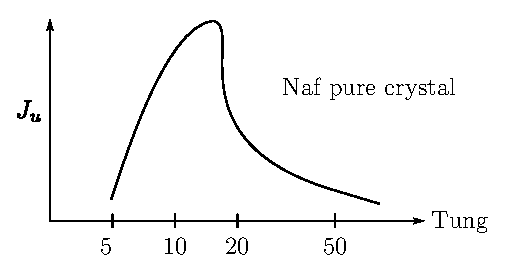
\includegraphics{images/lecture20/fig6.eps}
\end{figure}

Al low temperature Umklapp process become ineffective and dimension effect becomes dominant.

$l\sim D$ (diameter of the specimen)

$\therefore \ k\sim C\sim D$ only temperature dependent term is `$C$'.

At low $T$, $C$ goes as $T^{3}$ and hence thermal conductivity too goes as $T^{3}$.
